\chapter{MeDSpace}

In this chapter we will present the developed system MeDSpace (\textit{abbr.} for Medical Dataspace) whereas in the next chapter we will look at more implementation specific details.

The purpose of MeDSpace is to provide a distributed test environment of medical datasources. The focus thereby is the provision of a keyword search functionality over medical datasources. 
As distributed keyword search is the foundation for every Dataspace system, MeDSpace can be used as a starting point for a much more evolved dataspace or as a framework for implementing advanced dataspace functionality.
Although the system uses medical datasources for its test data, the system is general enough to be used for other dataspace-related projects or systems, that need keyword search functionality over a set of multiple heterogenous (multimedia) datasources. 

In figure \ref{MeDSpaceOverview} the overview of the MeDSpace system is illustrated.
\begin{figure}[H]
	\begin{center}
	%\hspace*{-1cm}
		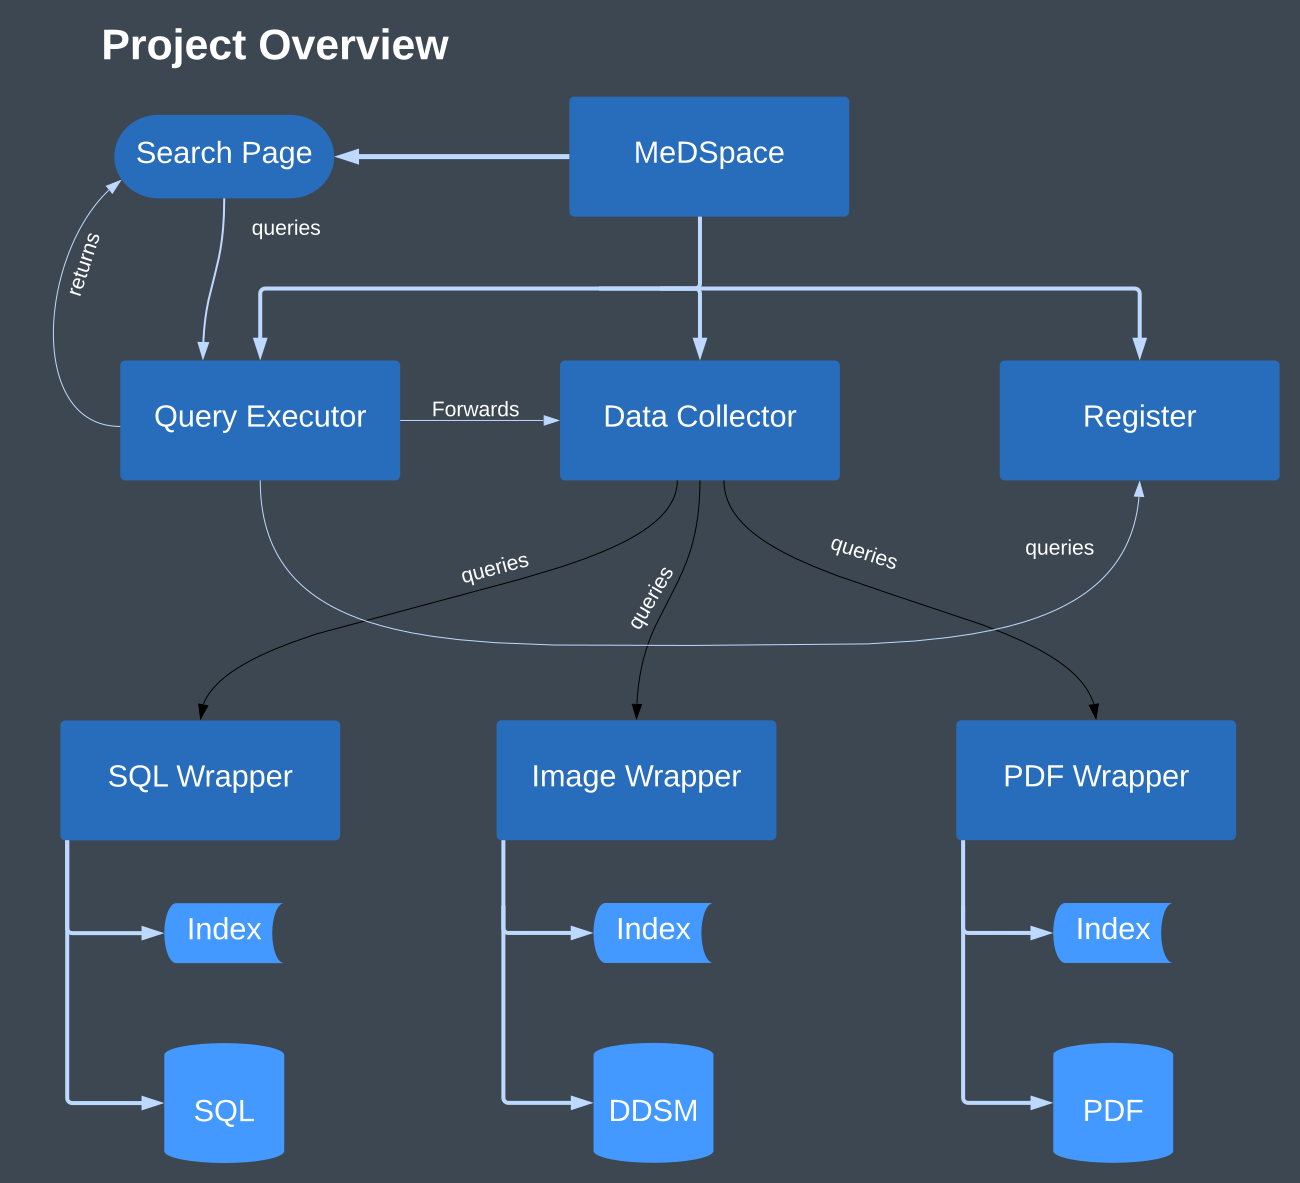
\includegraphics[scale=0.145]{figures/MeDSpace-Overview.png}
	\end{center}
	\caption{MeDSpace Project overview}
	\label{MeDSpaceOverview}
\end{figure} 

The system can roughly be divided into a \emph{wrapper} and a \emph{global MeDSpace} category: The \emph{wrapper} category includes everything from managing the data of a specific datasources (e.g. from a relational database). 
Whereas the \emph{global MeDSpace} category comprises datasource management and services on a global view.  The modules belonging to this category are the \emph{Register}, the \emph{Data Collector}, the \emph{Query Executor}, and the \emph{Search Page}.  

Now, we want look at the requirements met by MeDSpace. Therefore we look at the purposes of each module of the system.

\section{General} 
MeDSpace uses RDF \cite{w3RDF} as its canonical data model. Although a dataspace system is not restrict to use a specific data model, it simplifies the complexity of data management.
Furthermore RDF is proposed to be used for Linked Data \cite{LinkedData} in the Semantic Web field. Although a different research field, both fields face semantic data-integration.

All wrappers and the register have configuration files. These configuration files use XML and each configuration file has a corresponding \emph{XML Schema Definition} (XSD)\cite{w3XMLSchema} file, that is used to validate the configuration file. This allowed us to generate automatically Java classes out of the XSD files using \emph{Java Architecture for XML Binding} (JAXB) \cite{JAXB}.


\subsection{Importance of unicode}

A dataspace includes data sources possibly spread around the globe. It is near inferring to support a wide area of different languages. In terms of character sets, it is therefore necessary to use a unicode encoding.
Unicode is a system assigning each character a unique code point and it is designed to support the worldwide interchange, processing and display of texts written in different languages\cite{UnicodeStandard}.\newline
There exist several encodings for unicode. The more well known are the UTF and UCS encoding families. In the draft of HTML5 it is advised to use UTF-8 for new web pages\cite{HTML5Rec}. 
Thus, to simplify processing, we follow the recommendation and use UTF-8 throughout the dataspace. If a data source doesn't use UTF-8, it is the task of its wrapper to do a proper conversion to UTF-8.

\subsection{Keyword query language convention}
As already previously told, the one service that every wrapper has to implement is the keyword search functionality. In order to search for specific keywords, it is important to define a convention how the keyword search should work, since there are several possibilities. E.g. if a query is posed with two keywords, should a query be created for all results that contains both keywords or is it enough if one of the keywords is contained? Should boolean operators be allowed (AND, OR, NOT)? 

The design decision is at follows: Rudimentary keyword search functionality suffices and several keyword searches have to be interpreted in an 'AND like' manner by default, i.d. all of the stated keywords have to occur to fulfill the query condition. Additionally, the user should be able to use an 'OR' operator instead. This option is included in the search page.

The reasons are, that no complex global query language is necessary, that all wrappers have to implement which leads to much more flexible implementation decisions. As wrappers can provide as many services as they like it is easy to provide a much more powerful keyword search service. So this design decision doesn't restrict the power of a wrapper.

We think, that it is more likely for a user to want results that include all stated keywords and not only one of it. So we decided to use the 'AND' operator by default. In certain cases it should be useful to use the 'OR' operator, so we added it, too.

\section{Wrappers}
Each local datasource has its own wrapper. The wrapper is similar to the wrappers used in a mediator-based system, but provides dataspace specific functionality: the wrapper...
\begin{itemize}
	\item manages the data exchange between the datasource and extern MeDSpace services.
	\item provides keyword search functionality (if the datasource doesn't provide it itself already). Therefore it creates an index of the data of the wrapped datasource and maintains it. 	
	\item converts search results from the datasource to the canonical data model.
	\item registers and deregisters the datasource from MeDSpace by communicating with the \emph{Register} module. The wrapper informs the register what services the datasource and the wrapper provide.
	\item overcomes technical, syntactic and data model heterogeneity. 
\end{itemize}

Thereby the \emph{SQL Wrapper} is responsible for wrapping a relational database containg data created with the \emph{Patient Data Generation Framework} (PDGF) tool created by Schmiedbauer \cite{SchmidbauerBachelorThesis}. The \emph{Image Wrapper} provides access to case files of \emph{Digital Database for Screening Mammography} (DDSM)\cite{DDSM} and the \emph{PDF Wrapper} maintains a set of pdf files that were created specific for this system: the pdf files contain data based on Schmidbauer's test data.

\section{Register}
The Register holds a list of active datasources that can be queried. Therefore it provides functionality so that wrappers can register and deregister a datasource. In order to know what services are provided by each datasource, the register also keeps records of these services. This allows other modules to use services of any datasource.
\section{Query Executor}
The task of the \emph{Query Executor} is to accept a given keyword search query, transform this query to a service call and instructs the \emph{Data Collector} module to call the keyword search service for each registered data sources. To know which datasources are registered, this module communicates with the \emph{Register} module. After the \emph{Data Collector} has collected the query results of all datasources the \emph{Query Executor} adds the search query to its query cache and returns the collected search result to the caller who requested the \emph{Query Executor}. On the next request, the cached query result will be returned without querying the datasources if no 'cache miss' has been occurred.

Note: It is not the task of the \emph{Query Executor} to actually collect the search result from the datasources. That is done by the \emph{Data Collector}. It does only instruct the \emph{Data Collector} to do the collecting.

\section{Data Collector}
The \emph{Data Collector} provides services that allow to query a specific  datasource and store the query result into a specific RDF repository that is maintained by this module. Furthermore the \emph{Data Collector} allows other modules to create and remove a repository that is coupled with a specific search query. This allows the \emph{Query Executor} to merge the search results of all datasources into a seperate RDF repository. Then, again the \emph{Query Executor} is able to delete the repository if the associated and cached query result should be deleted. 

\section{Search Page}
Represents the \emph{graphical user interface} (GUI) so that a user can easily interact with the MeDSpace system using a common browser. It provides a page for stating and sending keyword searches, allows the user to display the search result in the browser or download it as a file. Furthermore the search page allows the user to inspect the list of the current registered datasources and it allows to delete the query cache.

\chapter{Implementation}
In this chapter we focus on implementation details of the MeDSpace system: What technology is used, how and why the implementation is structured, and also on details that developers should know to use the system rightly.

\section{Used technologies}

In this section we want to present the technologies that are used by MeDSpace.

\subsection{Programming language - Java}
MeDSpace is written completely in Java 8. The reason for java are diverse: its platform independence is something very helpful in a heterogeneous environment. Java with its JIT compiler runs nearly as fast as C++ and outperforms several other languages. Performance is something that didn't is something too important, but it should not be neglected, especially as the system has to handle potentially very large data sets. And last but not least, Java has great library support for Web development. 
Of course, other languages could be used, too. But Java is definitive a good choice.

\subsection{Resource Description Framework}

The \emph{Resource Description Framework} (RDF) \cite{w3RDF} is used as the canonical data model in MeDSpace. RDF is a graph-based abstract data model. With abstract, we mean it is a conceptual data model, so RDF says nothing about serializing data. But there exists plenty serialization formats that can be used to serialize RDF data. A popular RDF serialization format is Turtle \footnote{\url{https://www.w3.org/TR/turtle/}}, that is known to be easy human readable.
It facilitates merging data expressed in different schemas, as objects are identified by URIs and with the help of ontologies, semantic data integration can be performed by logical inference. 

Figure \ref{RdfTriple} shows how rdf data is structured.
\begin{figure}[H]
	\begin{center}
		\includegraphics[scale=0.75]{figures/rdf-graph.pdf}
	\end{center}
	\caption{A predicate connects two nodes (Subject, Object) forming an RDF Triple}
	\label{RdfTriple}
	\footnotemark
\end{figure}
\footnotetext{\url{https://www.w3.org/TR/rdf11-concepts/rdf-graph.svg}}

RDF data consists of resources, which are the nodes of the rdf graph, and predicates, which are directed edges between the resources. So rdf is a directed graph. 

Resources can be IRIs, literals and blank nodes. 
Resources with an IRI are identified through its IRI. Two resources with the same IRI are supposed to be equal.
Blank nodes are also called anonymous resources, as they specify the existence of a thing, but it is not identifiable. So blank nodes are always unique.
Literals are used for values like numbers, strings or a date aren't identifiable, too.
Predicates are always IRIs and can also be resources. They are also identified by their IRIs.

The idea of RDF is, to represent data in form of triple statements, that consists of two resources (subject and object in figure \ref{RdfTriple}) and a predicate. The statement 'A has a property B' could be expressed in RDF with two resources A (the subject) and B (the object) and a predicate with an IRI, that should form the 'has' predicate. It should be noted that a subject can be an IRI or a blank node, but not a literal. As a result about a literal no statements can be made.


In MeDSpace we used the RDF4J framework \cite{RDF4J}, that enables to read and write RDF content from within Java. Originally we planned to use Apache Jena \cite{Jena}, but it wasn't possible for us to convert the RDF data into an appropriate input and output stream classes without the Jena PipedRDFIterator class \footnote{\url{https://jena.apache.org/documentation/javadoc/arq/org/apache/jena/riot/lang/PipedRDFIterator.html}}, that unfortunately creates a new thread for processing the rdf triples. But that isn't an option for us, as this solution doesn't scale well.


\section{Setting up databases}


\subsection{Setting up a MySQL data source}

To setup a MySQL datasource get a recent stable MySQL community server\footnote{\url{https://www.mysql.de/downloads/}} 
and install it for your target platform. Additionally you will need the Connector/J components, the official JDBC driver for MySQL. 

At time of writing, the most recent stable versions are the community server 5.7.17 and the Connector/J 5.1.41. These versions are used for the thesis project and all following commands are related on them. If you're using 
different versions, assure that the instructions are adapted properly. As a detailed installation instruction for all supported platforms would break the mold, the reader is encouraged to consult the official 
manual\footnote{\url{https://dev.mysql.com/doc/}}. 
Assure that the MySQL binary folder is integrated into your class path, so that you can access it globally in a shell/command line. Although not necessary it is recommended for security reasons 
to set a password for the root user\footnote{\url{https://dev.mysql.com/doc/refman/5.7/en/default-privileges.html} , \url{https://dev.mysql.com/doc/refman/5.7/en/resetting-permissions.html}}. 
After installing the server, do postinstallation setup and testing\footnote{\url{https://dev.mysql.com/doc/refman/5.7/en/postinstallation.html}}. 

To support UTF-8, set in your my.cnf 

\begin{codebox}
	default-character-set = utf8
\end{codebox}

in the mysql section and

\begin{codebox}
	character-set-server=utf8\newline
	collation\-server=utf8\_general\_ci
\end{codebox}

in the mysqld section. Then restart the mysqld daemon. In the following, it is assumed, that you have a running MySQL server now that can be accessed via shell/command line. Before you connect to the MySQL server, you should assure that the application you use for connecting is using UTF-8 for user input and sending statements. So, validate that your shell/command line is using UTF-8. E.g. on windows system (before Windows 10) the command line isn't using UTF-8 by default
\footnote{To set the encoding to UTF-8 on the windows command line, change the active code page to 65001 and set 'Lucida Console' as the displaying font. In contrast to the font, the code page is only active for the current console session. But you can automate this command with a AutoRun setting. For more information see \url{https://blogs.msdn.microsoft.com/oldnewthing/20071121-00/?p=24433}}.  
Now try to connect to the database as the user root:

\begin{codebox}
	mysql -u root -p 
\end{codebox}

If you've done all right, you should be connected to the database after entering and confirming the password, that you've previously stated for the user root.

The next step is to validate, that UTF-8 is indeed continuously used. Execute:

\begin{codebox}
	SHOW VARIABLES LIKE 'char\%';
\end{codebox}

and check, that the variables \emph{character\_set\_client}, \emph{character\_set\_connection}, \emph{character\_set\_database}, \emph{character\_set\_results}, \emph{character\_set\_server} and \emph{character\_set\_system} are all set to utf8.
Basically, these variables are used to interpret and write data consistently in UTF-8. More information about the stated variables can be found on the manual
\footnote{\url{https://dev.mysql.com/doc/refman/5.7/en/server-system-variables.html\#sysvar_character_set_client}}.

The next step is to initialize the data source with a database and some content. Further we need a user which is used by the wrapper to communicate with the data source. The wrapper needs no writing rights and indeed we don't want it to change the data, so following the security rule 'As few rights as possible' we grant that user only reading rights for fetching data. The commands for initializing the data source and creating a read-user are in the file \textbf{init\_mysql.sql} which is located in the appendix data in the folder \textbf{implementation/SQL/mysql}.

To execute commands from a file, execute while logged in as the root user:

\begin{codebox}
	SOURCE \emph{path\_to\_sql\_file};
\end{codebox}

where \emph{path\_to\_sql\_file} is the full (absolute or relative) path to the sql file.
Per default, the created database will be named \textbf{medspace} and the read-user will be called \textbf{medspace\_client}. If you want edit the init.sql file, beware that the file is encoded in UTF-8. As we instructed mysql to use UTF-8 in every case, this is encoding is required. Assure that your file editor saves the file in that encoding, too.


\section{Wrappers}

As described in Chapter \ref{chapter_dataspaces}, a wrapper is  an interface between the datasource and the dataspace. The wrapper can provide any number of services to access the data of the datasource, but the one service, that every wrapper has to implement, is the keyword search.
In the thesis' project there are three datasources: A SQL database, a pdf file server and a SQL multimedia database serving image files. The SQL database and the multimedia image database contain
structured data while the pdf file server contains semi-structured data.
The following sub sections describe the functionality and implementation of the wrappers for the three datasources in detail.

\subsection{SQL Wrapper}

The task of the SQL Wrapper is to convert the SQL data into rdf and providing a keyword search functionality, as SQL databases doesn't provide such a functionality.

At first we want to look at the conversion from sql to rdf. To do this, the wrapper implements a specialized version of the D2rMap language. D2rMap was designed by Chris Bizer and is  a declarative language to describe mappings between relational databases schemata and OWL/RDFS ontologies\cite{D2rMap_aDatabaseToRdfMappingLanguage}.

D2rMap is a general purpose language to export any sql data to rdf. To better suit the needs for a dataspace wrapper, the language was changed. The changed language is called MeDSpace D2rMap and its language specification can be found in the appendix.

The mapping is done as follows: At first the user specifies mappings in a config file. Each mapping is used to create RDF instances of a certain type. The mapping contains a SQL query, that represents all the data, that is necessary to create the instances. Furthermore, in the mapping are columns specified, that are used to create unique IDs for the created RDF instances.
The next step is to fetch the sql data and to group the record set according to the fore mentioned columns. Now, each row of the grouped record set represents a rdf instance, so the instances can be created. The last step is the creation of the property statements. Important to note is the seperation of the last two steps. Through the seperation it is possible to reference other rdf instances (from the same mapping or another). The mapping process is visualized in figure \ref{D2rMappingProcessFigure}.

\begin{figure}[H]
	\begin{center}
		\includegraphics[width=0.75\textwidth]{figures/MappingProcess.pdf}
	\end{center}
	\caption{The D2r mapping process; Taken from \cite{D2rMap_aDatabaseToRdfMappingLanguage}}
	\label{D2rMappingProcessFigure}
\end{figure}

After discussing the SQL to RDF mapping, we look at the keyword search, now:
Mainly there are two possibilities, to implement a keyword search functionality:
\begin{itemize}
	\item {Construct a keyword search query in SQL and let the database answer the query.}
	
	\item {Use a keyword search engine that answers the query based on an external index}
\end{itemize}

At first glance, the first option sounds obviously simple, but after implementing it showed several disadvantages: SQL is not designed to provide search functionality based on keywords. SQL uses the \textbf{\emph{LIKE}} operator for pattern matching. But in order to do a Full-text search, the SQL Query executor cannot use any index resulting in poor query answer performance. Another problem of \emph{LIKE} is, that there is no way to define, that only whole words should be searched and not just sub word matching. Whole word matching is very important, as e.g. a user searching for data about male patients should not also get data about female patients.
As a result, the \emph{LIKE} operator is not suitable for a proper keyword search service as expected to be provided by a dataspace wrapper. Several SQL database vendors provide often own solutions for Full-Text search queries. But these solutions have often other restrictions as e.g. only column fields having the datatype \emph{TEXT} (on MySQL) and the fields have to specified to be fulltext fields, so that the SQL engine is able to create an index for it (at MySQL databases at least).
A Wrapper could use vendor specific services but that would exclude other SQL database vendors, obviously. 

The second option doesn't rise the aforementioned issues of option one. For the Wrapper a keyword searcher was implemented using the fulltext search engine Apache Lucene Core \footnote{\url{https://lucene.apache.org/core/}}. The advantage of using Lucene is it's high-performance and scaling of keyword searches over large data sets. Additionally it allows a fine granular configuration about the query construction and sorts automatically the query result by relevance (so called query result ranking). \\
The major disadvantage of using lucene is that the SQL data have to be extracted and indexed outside the database. If the data changes or rows are added resp. deleted, the index has to be updated accordingly. The update process can be very complex, as not only new data has to be indexed resp. existing data has to be removed, but also data that references the deleted or new data that depends on it.\\
A simpler but obviously slower solution is to reindex the whole data set. Reindexing the whole data set is only advised if updates occur not that often or if it is acceptable if the wrapper updates the index not instantly and thus provides potentially outdated data.

The decision which method is more suitable depends primarily on the use case and the domain. As the project is designed to be used as a test suite for medical datasources and medical science, it is acceptable if the data is outdated to some degree and will be updated not frequently. Changes on the datasource haven't to be updated in near-realtime. Having this in mind, the preferred method for the keyword search functionality clearly is using Apache Lucene Core, as the  advantages clearly outweigh its disadvantages. Thus, a full functional keyword searcher was implemented powered by Lucene.

\subsection{Image Wrapper}
fgfg
\subsection{PDF Wrapper}

\section{Register}

\section{Keyword search}
\section{GUI}